% =====================================================================
%  Chapitre 1 -- Du MLP aux CNN
%  Partie c : les trois defauts du MLP, et la reponse des CNN
% =====================================================================

\begin{frame}{Les trois défauts structurels du MLP}
\begin{columns}[t]
\begin{column}{0.31\textwidth}
\begin{wbox}[1. Explosion des paramètres]
Un poids \emph{par pixel et par neurone}. On vient de le mesurer : 48 milliards
pour une photo. Rien ne peut être appris dans ces conditions.
\end{wbox}
\end{column}
\begin{column}{0.31\textwidth}
\begin{wbox}[2. Connexions spatialement absurdes]
Le réseau cherche des corrélations entre \emph{tous} les pixels, y compris entre
deux pixels opposés de l'image, qui n'ont rien à voir.
\end{wbox}
\end{column}
\begin{column}{0.31\textwidth}
\begin{wbox}[3. Dépendance à la position]
Chaque poids est lié à \emph{une} position précise. Le même motif placé
ailleurs n'est plus reconnu.
\end{wbox}
\end{column}
\end{columns}
\vspace{2mm}
\begin{kbox}[Le point commun]
Le MLP traite l'image comme une \textbf{liste de nombres sans structure}. Or
l'information utile d'une image est précisément \emph{dans} sa structure
spatiale : un œil, un bord, une texture.
\end{kbox}
\end{frame}

\begin{frame}{Ce que fait un œil humain : chercher des caractéristiques}
\begin{columns}[t]
\begin{column}{0.52\textwidth}
\begin{itemize}
  \item Face à un animal au loin, personne ne compare pixel par pixel.
  \item On parcourt la scène et on repère des \textbf{caractéristiques}
  (\emph{features}) : deux oreilles, des moustaches, un museau, des pattes.
  \item On conclut : « c'est un chat ».
\end{itemize}
\begin{kbox}[L'idée fondatrice]
Reconnaître, c'est détecter des \textbf{motifs locaux} puis les \textbf{combiner}.
C'est exactement ce que fera un CNN : d'abord des bords, puis des textures,
puis des parties d'objets.
\end{kbox}
\end{column}
\begin{column}{0.44\textwidth}
\begin{ebox}[Et pour détecter ces motifs ?]
La convolution. Un noyau bien choisi fait ressortir un bord, une texture,
une zone lumineuse.

\medskip
Le chapitre 2 en détaille le calcul ; pour l'instant, retenez le rôle :
\textbf{détecteur de caractéristiques locales}.
\end{ebox}
\end{column}
\end{columns}
\end{frame}

\begin{frame}{Première idée : la localité}
\begin{columns}[t]
\begin{column}{0.48\textwidth}
\centering
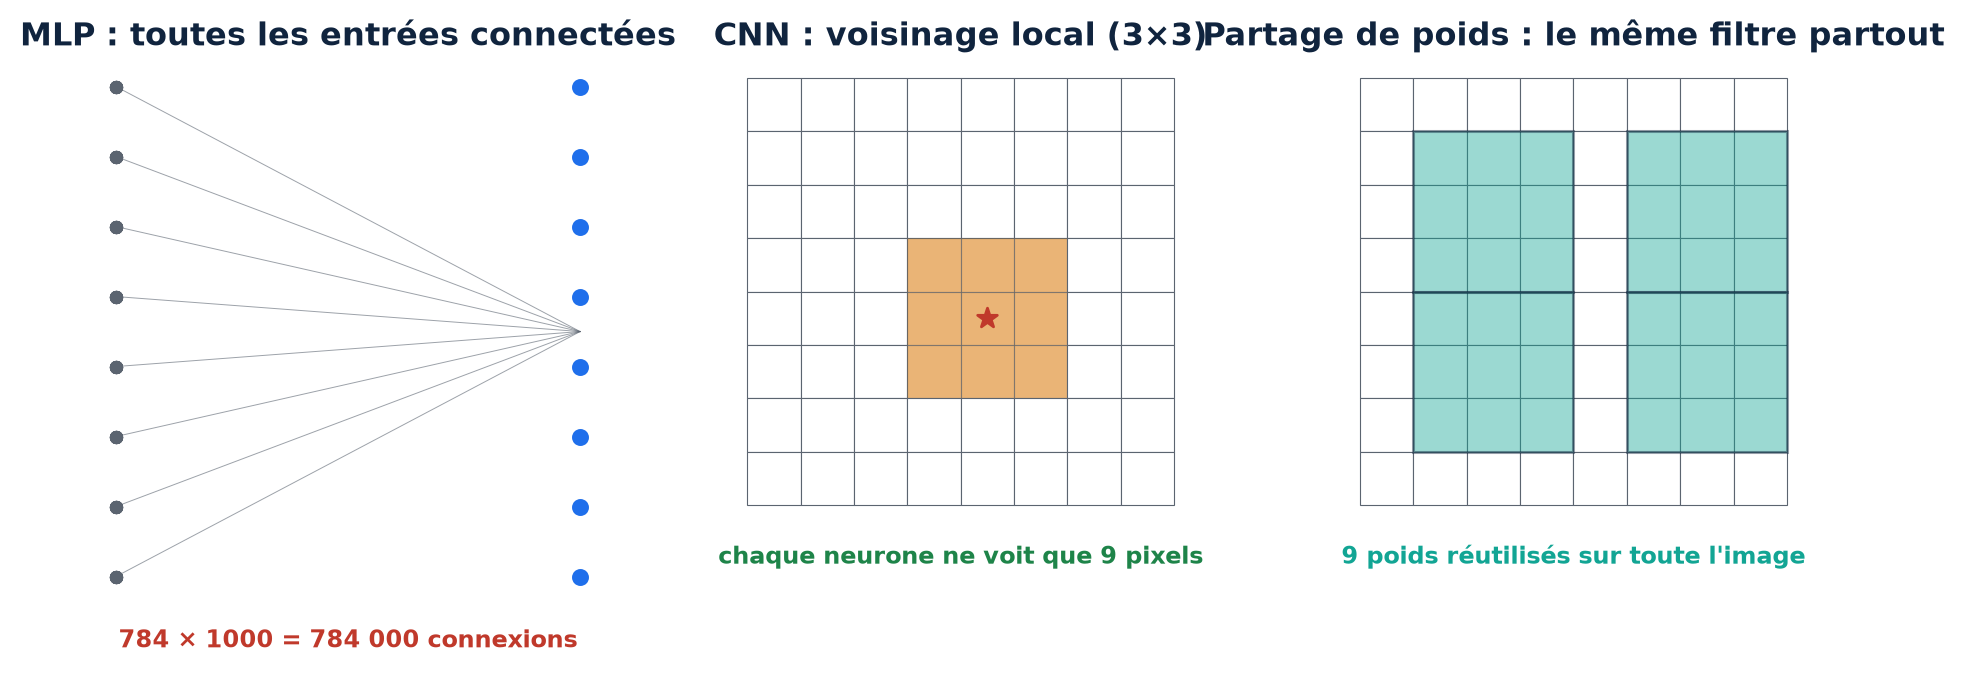
\includegraphics[width=\textwidth]{f03_localite_partage.png}
\end{column}
\begin{column}{0.48\textwidth}
\begin{itemize}
  \item \textbf{MLP :} chaque neurone voit $784$ pixels.
  \item \textbf{CNN :} chaque neurone ne voit qu'un \textbf{voisinage},
  par exemple $3 \times 3 = 9$ pixels.
  \item Deux pixels voisins portent une information commune ; deux pixels
  opposés, non.
\end{itemize}
\begin{kbox}[Voisinage = champ récepteur]
La petite zone vue par un neurone s'appelle son \textbf{champ récepteur}.
C'est la brique de tout le cours.
\end{kbox}
\end{column}
\end{columns}
\end{frame}

\begin{frame}{Deuxième idée : le partage de poids}
\begin{columns}[t]
\begin{column}{0.52\textwidth}
\begin{itemize}
  \item Le \textbf{même noyau} de $9$ poids balaie toute l'image.
  \item Il détecte donc le motif \emph{où qu'il soit}.
  \item Coût : $9$ poids, quel que soit le nombre de positions.
\end{itemize}
\begin{solbox}[Comparaison, pour une image $28 \times 28$]
\begin{center}
\begin{tabular}{@{}lr@{}}
\toprule
couche dense, $1\,000$ neurones & $784\,000$ paramètres \\
9 noyaux $3 \times 3$ ($9$ filtres) & $81$ paramètres \\
\bottomrule
\end{tabular}
\end{center}
\end{solbox}
\end{column}
\begin{column}{0.44\textwidth}
\begin{wbox}[Le prix à payer]
Un filtre donné ne détecte qu'\textbf{un type} de motif. Pour détecter des
bords horizontaux \emph{et} verticaux, il faut \textbf{plusieurs filtres} ---
d'où les « canaux de sortie » du chapitre 3.
\end{wbox}
\end{column}
\end{columns}
\end{frame}

\begin{frame}{Conséquence : l'invariance par translation}
\begin{columns}[t]
\begin{column}{0.55\textwidth}
\centering
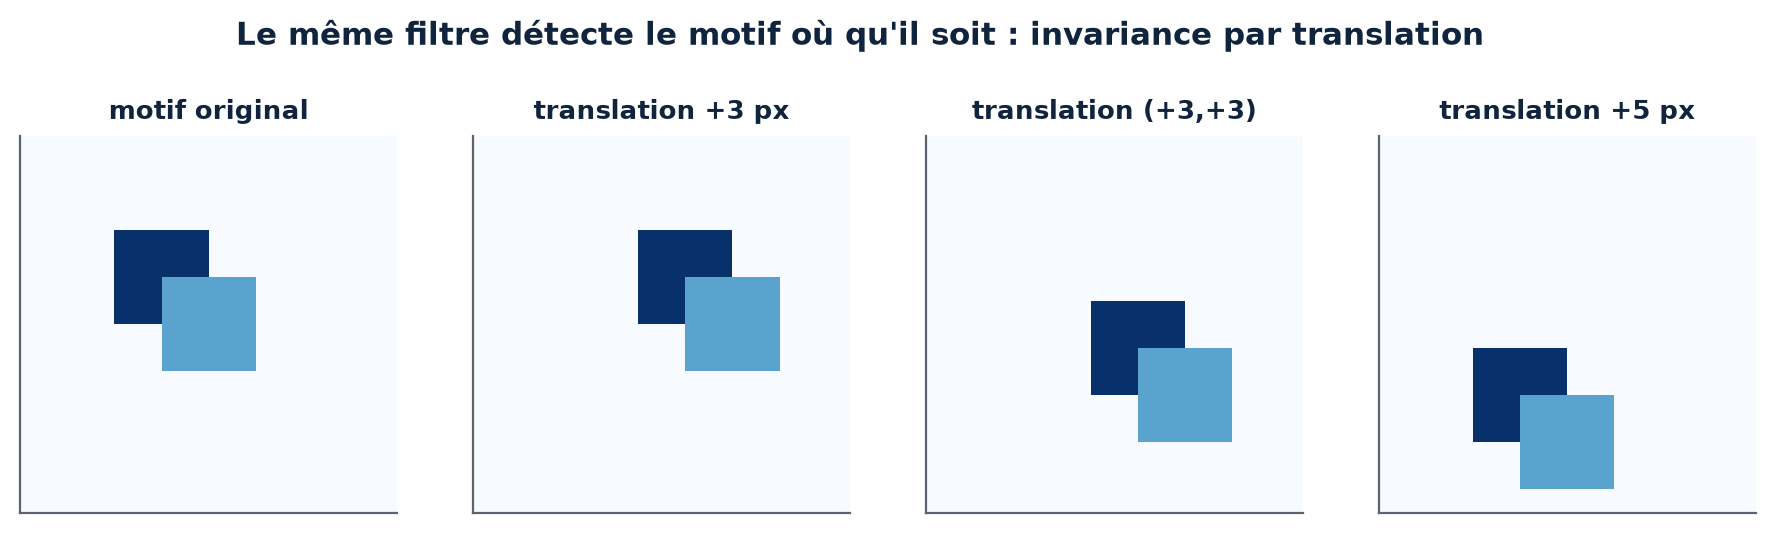
\includegraphics[width=\textwidth]{f04_invariance_translation.png}
\end{column}
\begin{column}{0.42\textwidth}
\begin{itemize}
  \item Le motif se déplace : la sortie du filtre se déplace avec lui,
  mais \textbf{reste identique}.
  \item Un pooling (chapitre 3) transformera ensuite cette « présence quelque
  part » en décision stable.
\end{itemize}
\begin{kbox}[Localité + partage = invariance]
C'est la propriété qui rend la reconnaissance d'images possible : un chat est
un chat, qu'il soit au centre ou dans un coin.
\end{kbox}
\end{column}
\end{columns}
\end{frame}

\begin{frame}{Quiz 2 --- localité et partage}
\begin{qbox}[Question 1]
Un noyau $3 \times 3$ sur une image en niveaux de gris contient combien de poids
apprenables ?
\begin{itemize}
  \item[(a)] 9 \quad (b) 784 \quad (c) cela dépend de la taille de l'image
\end{itemize}
\end{qbox}
\begin{qbox}[Question 2]
Le même noyau est appliqué à deux images : l'une où le motif est en haut à gauche,
l'autre où il est en bas à droite. Que peut-on affirmer ?
\begin{itemize}
  \item[(a)] Le filtre ne détecte rien dans le second cas
  \item[(b)] La carte d'activation montre le motif à la même position
  \item[(c)] La carte d'activation montre le motif à la position correspondante
\end{itemize}
\end{qbox}
\begin{qbox}[Question 3]
Pourquoi faut-il plusieurs filtres dans une couche convolutive ?
\begin{itemize}
  \item[(a)] Pour accélérer le calcul \quad (b) Parce qu'un filtre ne détecte qu'un
  type de motif \quad (c) Pour réduire la mémoire
\end{itemize}
\end{qbox}

% [fix] bloc deplace
\end{frame}
\begin{frame}{Quiz 2 --- localité et partage (suite)}
\begin{solbox}[Réponses]
\textbf{1.} (a) : 9 poids (+1 biais). \quad
\textbf{2.} (c) : la détection suit la position, c'est l'invariance par translation.
\quad
\textbf{3.} (b) : un noyau = un motif ; plusieurs motifs = plusieurs noyaux.
\end{solbox}
\end{frame}
